\documentclass[11pt,a4paper]{ctexart}
\usepackage[margin=1.5cm]{geometry}
\usepackage{graphicx}
\usepackage{booktabs}
\usepackage{array}
\usepackage{amsmath}
\usepackage{xcolor}
\usepackage{fancyhdr}
\usepackage{setspace}
\usepackage{titlesec}
\usepackage{caption}
\setlength{\columnsep}{0.6cm}
\linespread{1.15}

\pagestyle{fancy}
\fancyhf{}
\fancyhead[L]{\small S.H.I.T JOURNAL PREPRINT}
\fancyhead[R]{\small 本内容纯属整活}
\fancyfoot[C]{\thepage}

\titleformat{\section}{\large\bfseries\color{purple}}{\thesection.}{0.5em}{}
\titleformat{\subsection}{\normalsize\bfseries}{\thesubsection}{0.5em}{}

\begin{document}

\begin{center}
{\Large\bfseries\color{purple} 从“技术狂欢”到“生产力停滞”：\\
东亚 AI 工具热潮中的表演性采纳与结构性失配（2025--2026）}\\[0.5em]
李某某$^{1,*}$，王某某$^2$\\
\small 1. Department of Meme Economics, University of Excretion Technology\\
\small 2. Institute of Workflow Archaeology, Septic Tank Campus\\
\small *通讯作者: goushi@shitjournal.org
\end{center}

\vspace{0.4em}
\noindent\textbf{ABSTRACT / 摘要}\\
本文讨论一个看似热闹、实则虚空的现实：越来越多人在社交平台宣布“我接上 AI 了”，但真正可重复、可交付、可复盘的工作流并没有同步增长。基于东亚五地公开叙事样本（初始 $N=1204$；清洗后 $N=986$），我们构建 AS（接入展示强度）--FT（摩擦暴露时长）--DR7（7日留存）--IR（身份残留率）框架。结果显示：AS 与 DR7 显著负相关（$OR=0.662, p<0.001$），TaskClarity 显著正相关（$OR=1.681, p<0.001$），LearningCost 显著提高弃用风险（$HR=1.21, p<0.01$）。我们主张：AI 不是宗教，也不是考试。适配任务、适配人格、适配场景，才是长期有效的采纳策略。

\vspace{0.5em}
\noindent\textbf{INDEX TERMS / 关键词} AI 扩散；表演性采纳；平台激励；学习成本；数字劳动；反技术狂热

\vspace{0.5em}
\noindent\textbf{IMPACT STATEMENT / 影响声明}\\
我们反对两种极端：一种是“AI 无所不能”的新技术福音论，另一种是“不会用 AI 就要被淘汰”的焦虑营销。真正值得讨论的，不是追风速度，而是个体如何在有限认知资源里做清醒选择。

\section{INTRODUCTION / 引言}
2025--2026 的东亚互联网像一个持续增压的蒸汽锅：每一周都有新模型、新 Agent、新教程、新截图。有人晒效率翻倍，有人晒自动化接管人生，也有人在凌晨两点一边报错一边转发“明天一定 all-in AI”。

问题是：我们究竟在追赶什么？是生产率，还是一种“我没有掉队”的心理安全感？

在平台化传播里，技术很容易被包装成身份。你不必真的理解它，只需表现出你正在使用它。于是，“接入”被误当成“掌握”，“展示”被误当成“产出”，“热情”被误当成“能力”。这就是本文要讨论的核心：\textbf{表演性采纳（performative adoption）}。

\begin{quote}
\textit{如果一项技术首先让你更会发截图，而不是更会完成任务，那它此刻对你来说，可能更像社交货币，不像生产工具。}
\end{quote}

我们不反对 AI。相反，我们认为 AI 应当被认真使用。但“认真使用”意味着你有权慢下来、有权局部采用、有权拒绝不适配的工作流，而不是被群体节奏推着狂奔。

\twocolumn

\section{DATA \& METHODS / 数据与方法}
\textbf{样本来源：}东亚五地公开社媒/论坛/群聊 AI 采纳叙事。清洗后 $N=986$。由于公开表达样本偏向“高活跃用户”，本文结论更接近机制解释，不宜机械外推至总体人口。

\textbf{变量定义（通俗版）：}AS=前48小时“我接上了”式展示频率；FT=从准备上手到首个关键报错的小时数；DR7=第7天是否仍用同一工具完成同一任务；IR=停用后是否继续维持“在用 AI”身份信号。

\begin{equation}
\Pr(DR7=1)=\text{logit}^{-1}(\alpha+\beta_1 AS+\beta_2 FT+\beta_3 IR+\beta_4 TaskClarity+\beta_5 LearningCost+\gamma X)
\end{equation}

稳健性检验包含 DR14 替换、极端值 trimming、分地区子样本与 Cox 风险模型。本文只主张“相关与结构性关联”，不夸大为单向因果裁决。

\begin{table}[h]
\centering
\caption{主模型结果（Logit）}
\begin{tabular}{>{\raggedright}p{2.2cm}ccc}
\toprule
变量 & Logit系数 & OR & p值 \\
\midrule
AS & -0.412 & 0.662 & $<0.001$ \\
FT & -0.028 & 0.972 & 0.002 \\
IR & -0.365 & 0.694 & 0.010 \\
TaskClarity & 0.519 & 1.681 & $<0.001$ \\
LearningCost & -0.184 & 0.832 & $<0.001$ \\
\bottomrule
\end{tabular}
\end{table}

\section{RESULTS / 结果}
结果高度一致地指向一个朴素事实：任务定义越清晰，留存越高；展示冲动越强，留存越差。换句话说，真正起作用的不是“有没有用过 AI”，而是“是否把 AI 嵌进可重复流程”。

Figure 1--4 与表格口径一致：TaskClarity 是最稳定的正向项；AS 与 LearningCost 是稳定负向项。Figure 3 为机制示意，不替代主估计。

\begin{figure}[h]
\centering
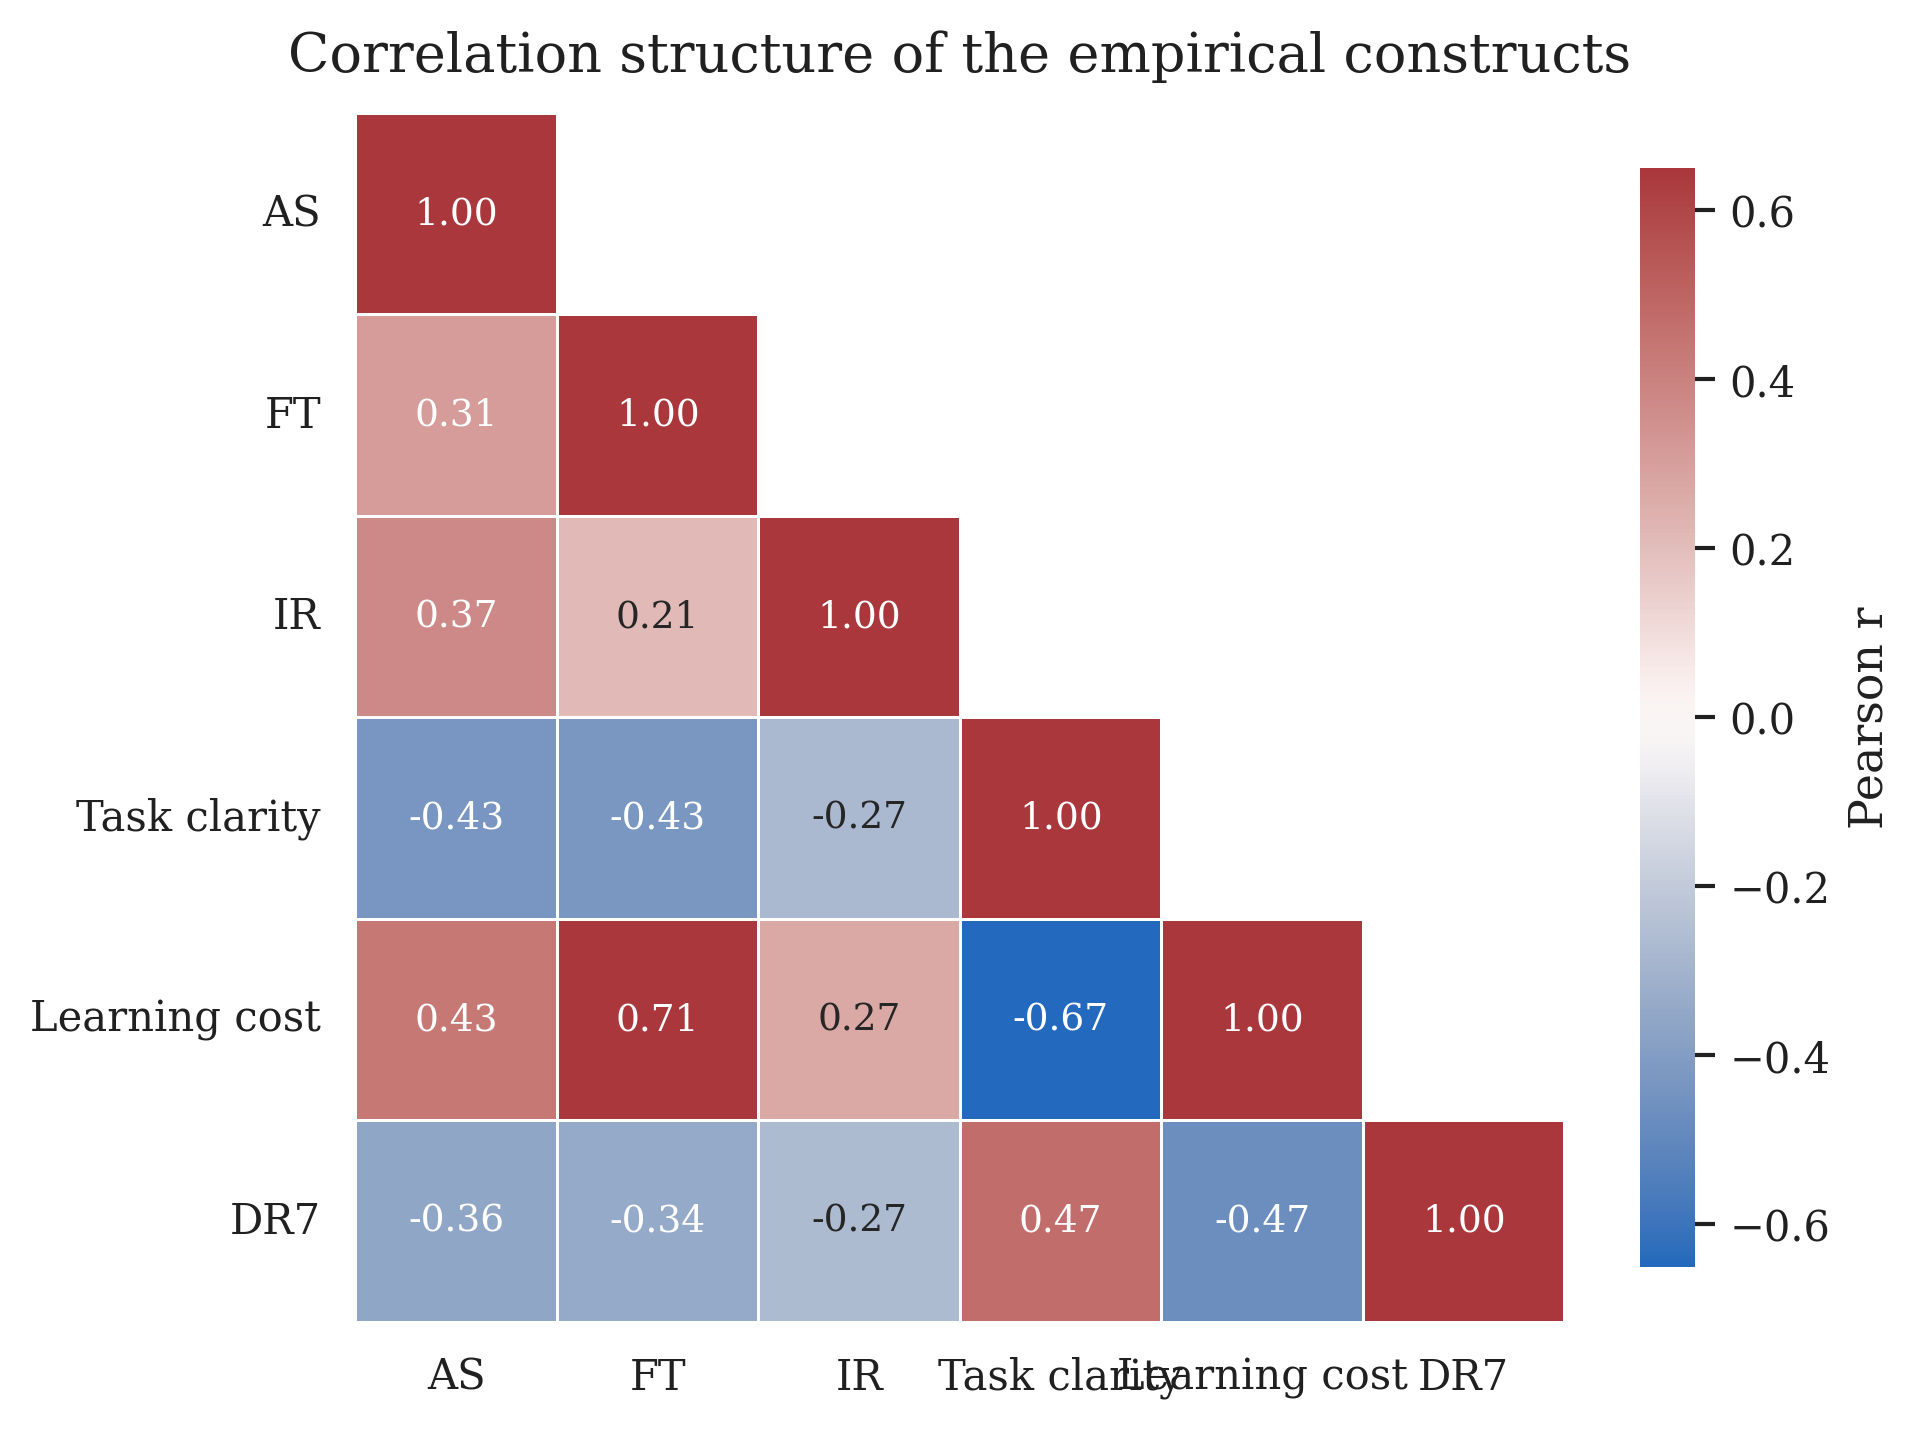
\includegraphics[width=0.95\columnwidth]{figures/fig1_correlation_heatmap.png}
\caption{变量相关热图}
\end{figure}

\begin{figure}[h]
\centering
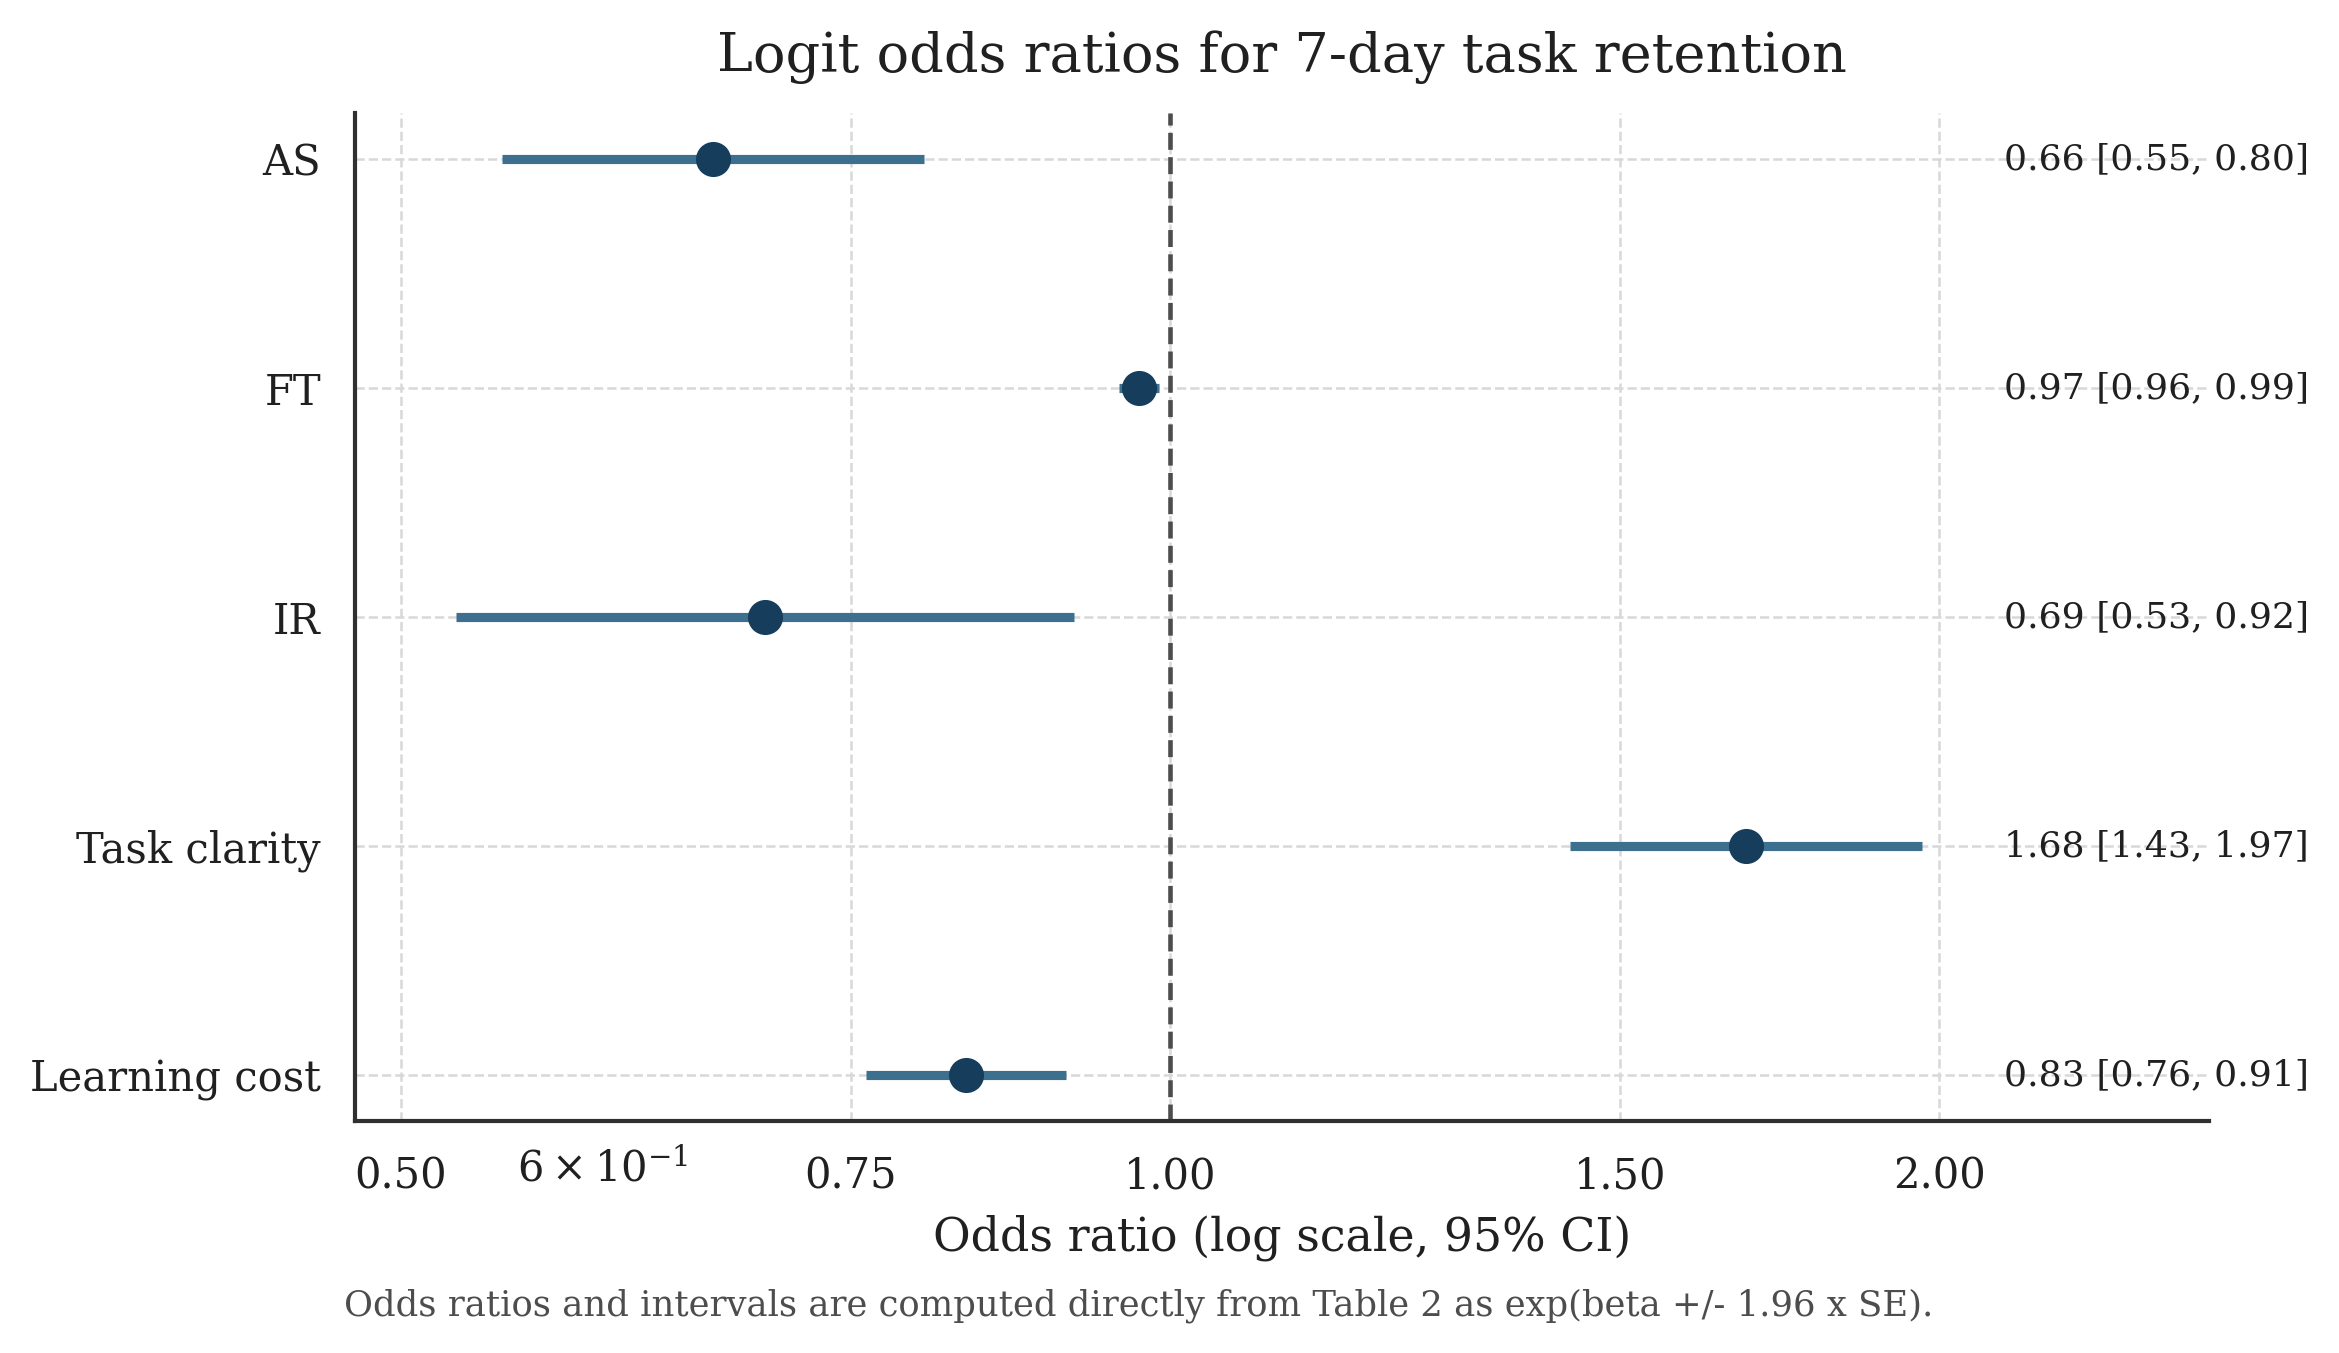
\includegraphics[width=0.95\columnwidth]{figures/fig2_logit_forest.png}
\caption{Logit OR 森林图}
\end{figure}

\begin{figure}[h]
\centering
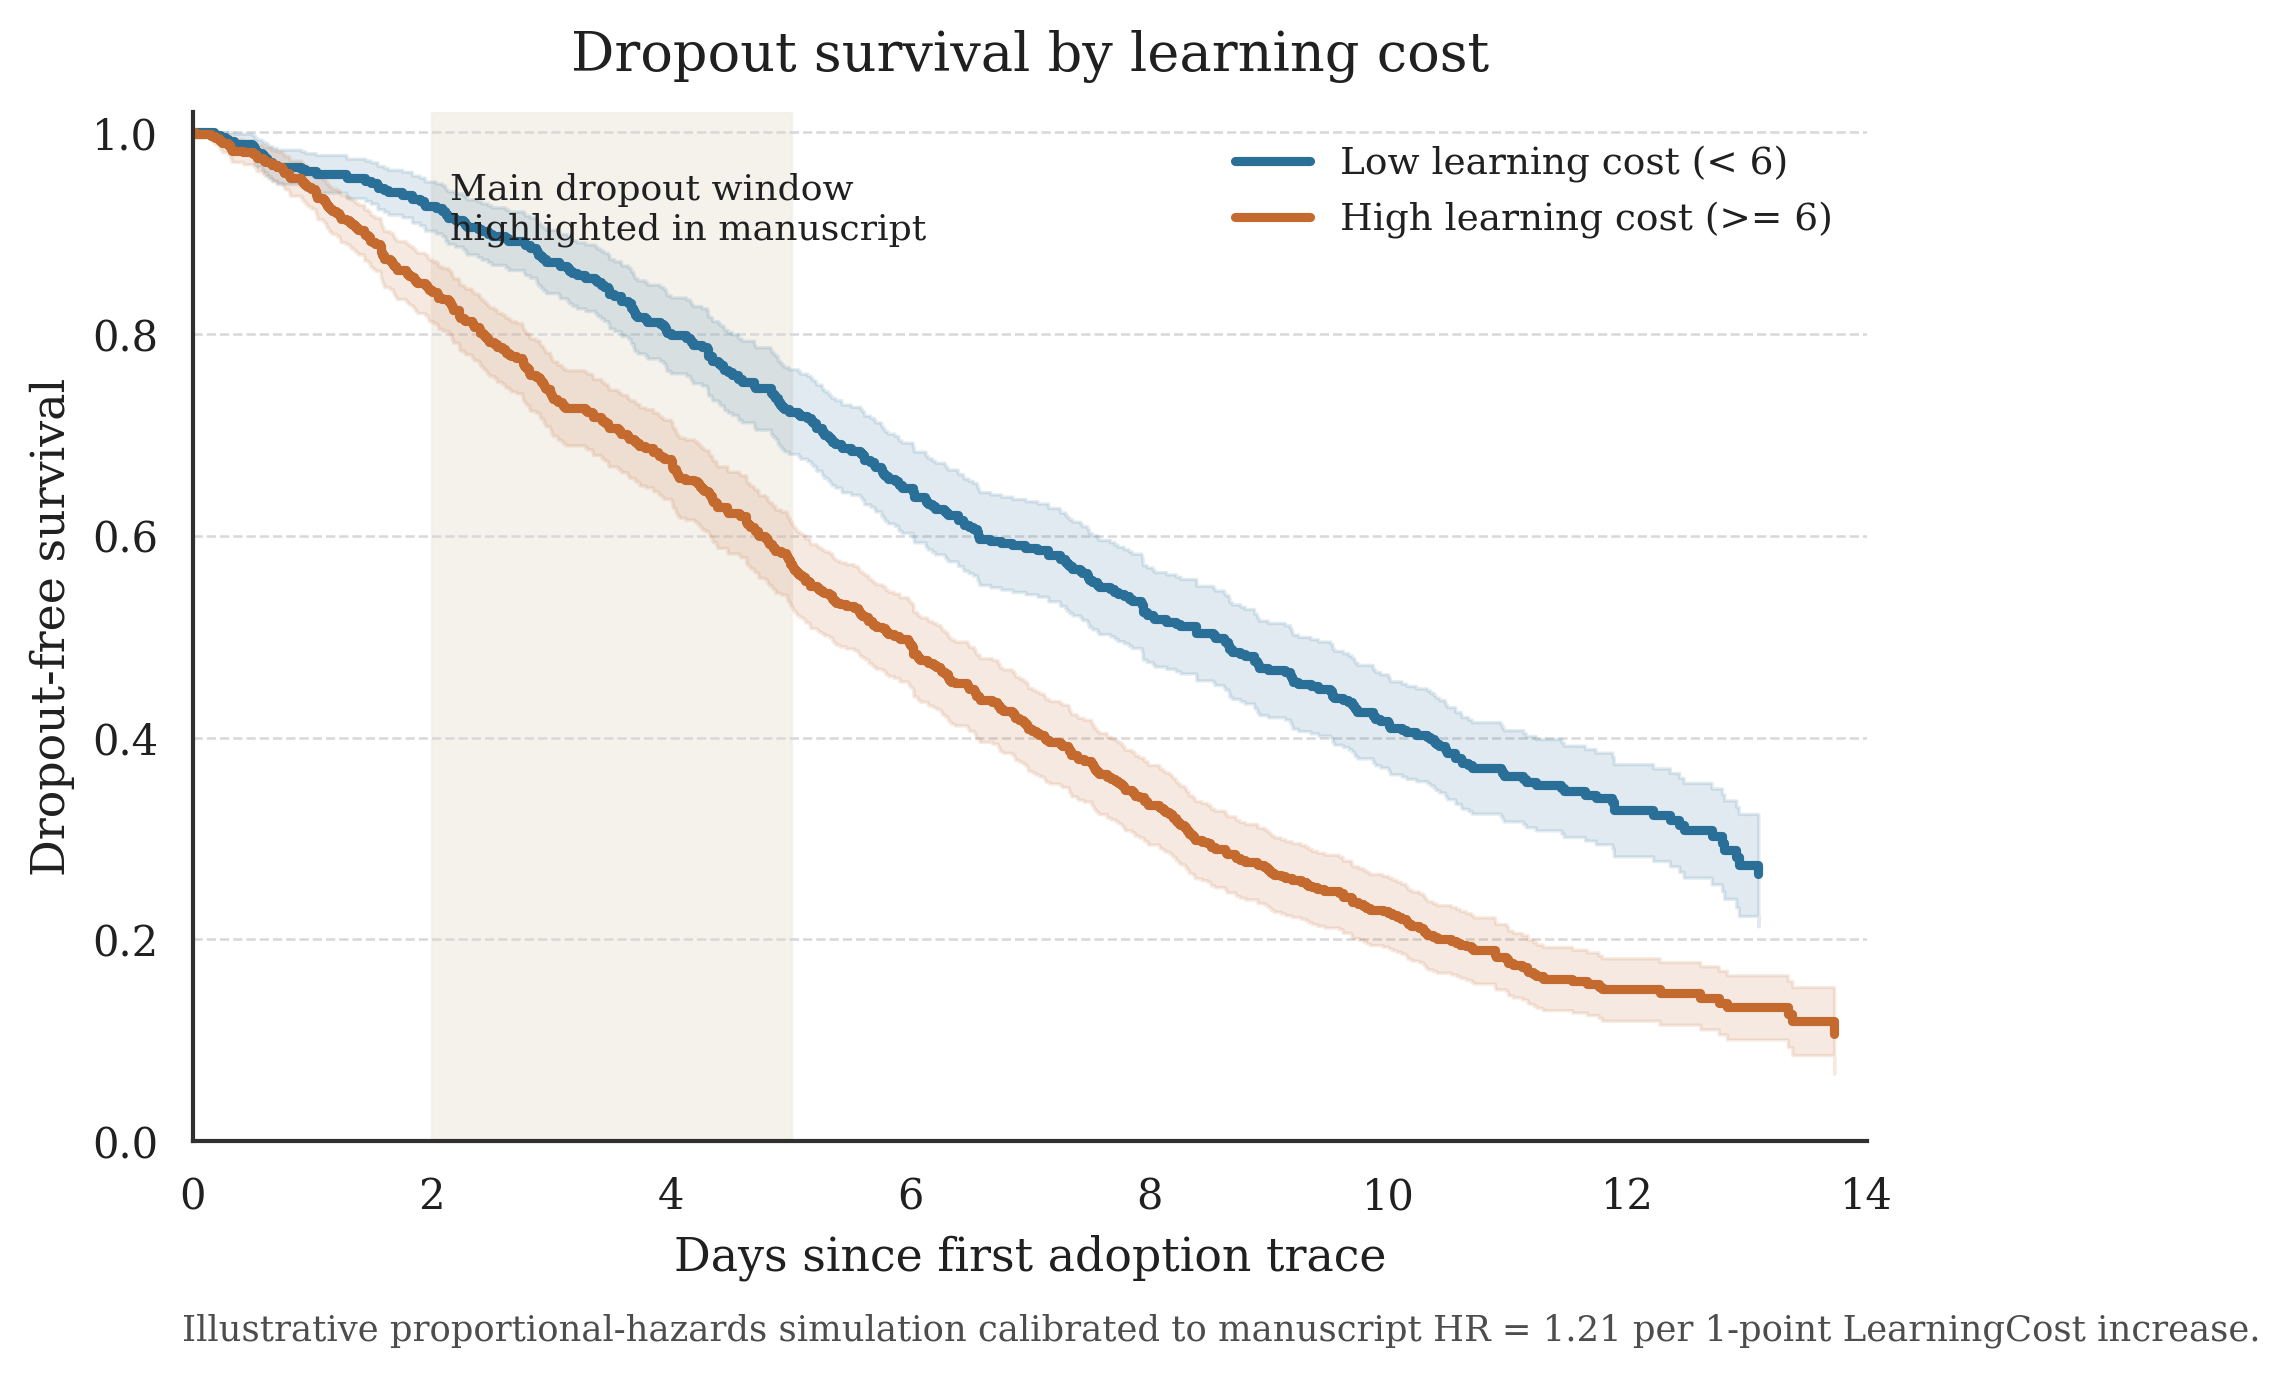
\includegraphics[width=0.95\columnwidth]{figures/fig3_survival_curve.png}
\caption{学习成本分组生存曲线（示意）}
\end{figure}

\begin{figure}[h]
\centering
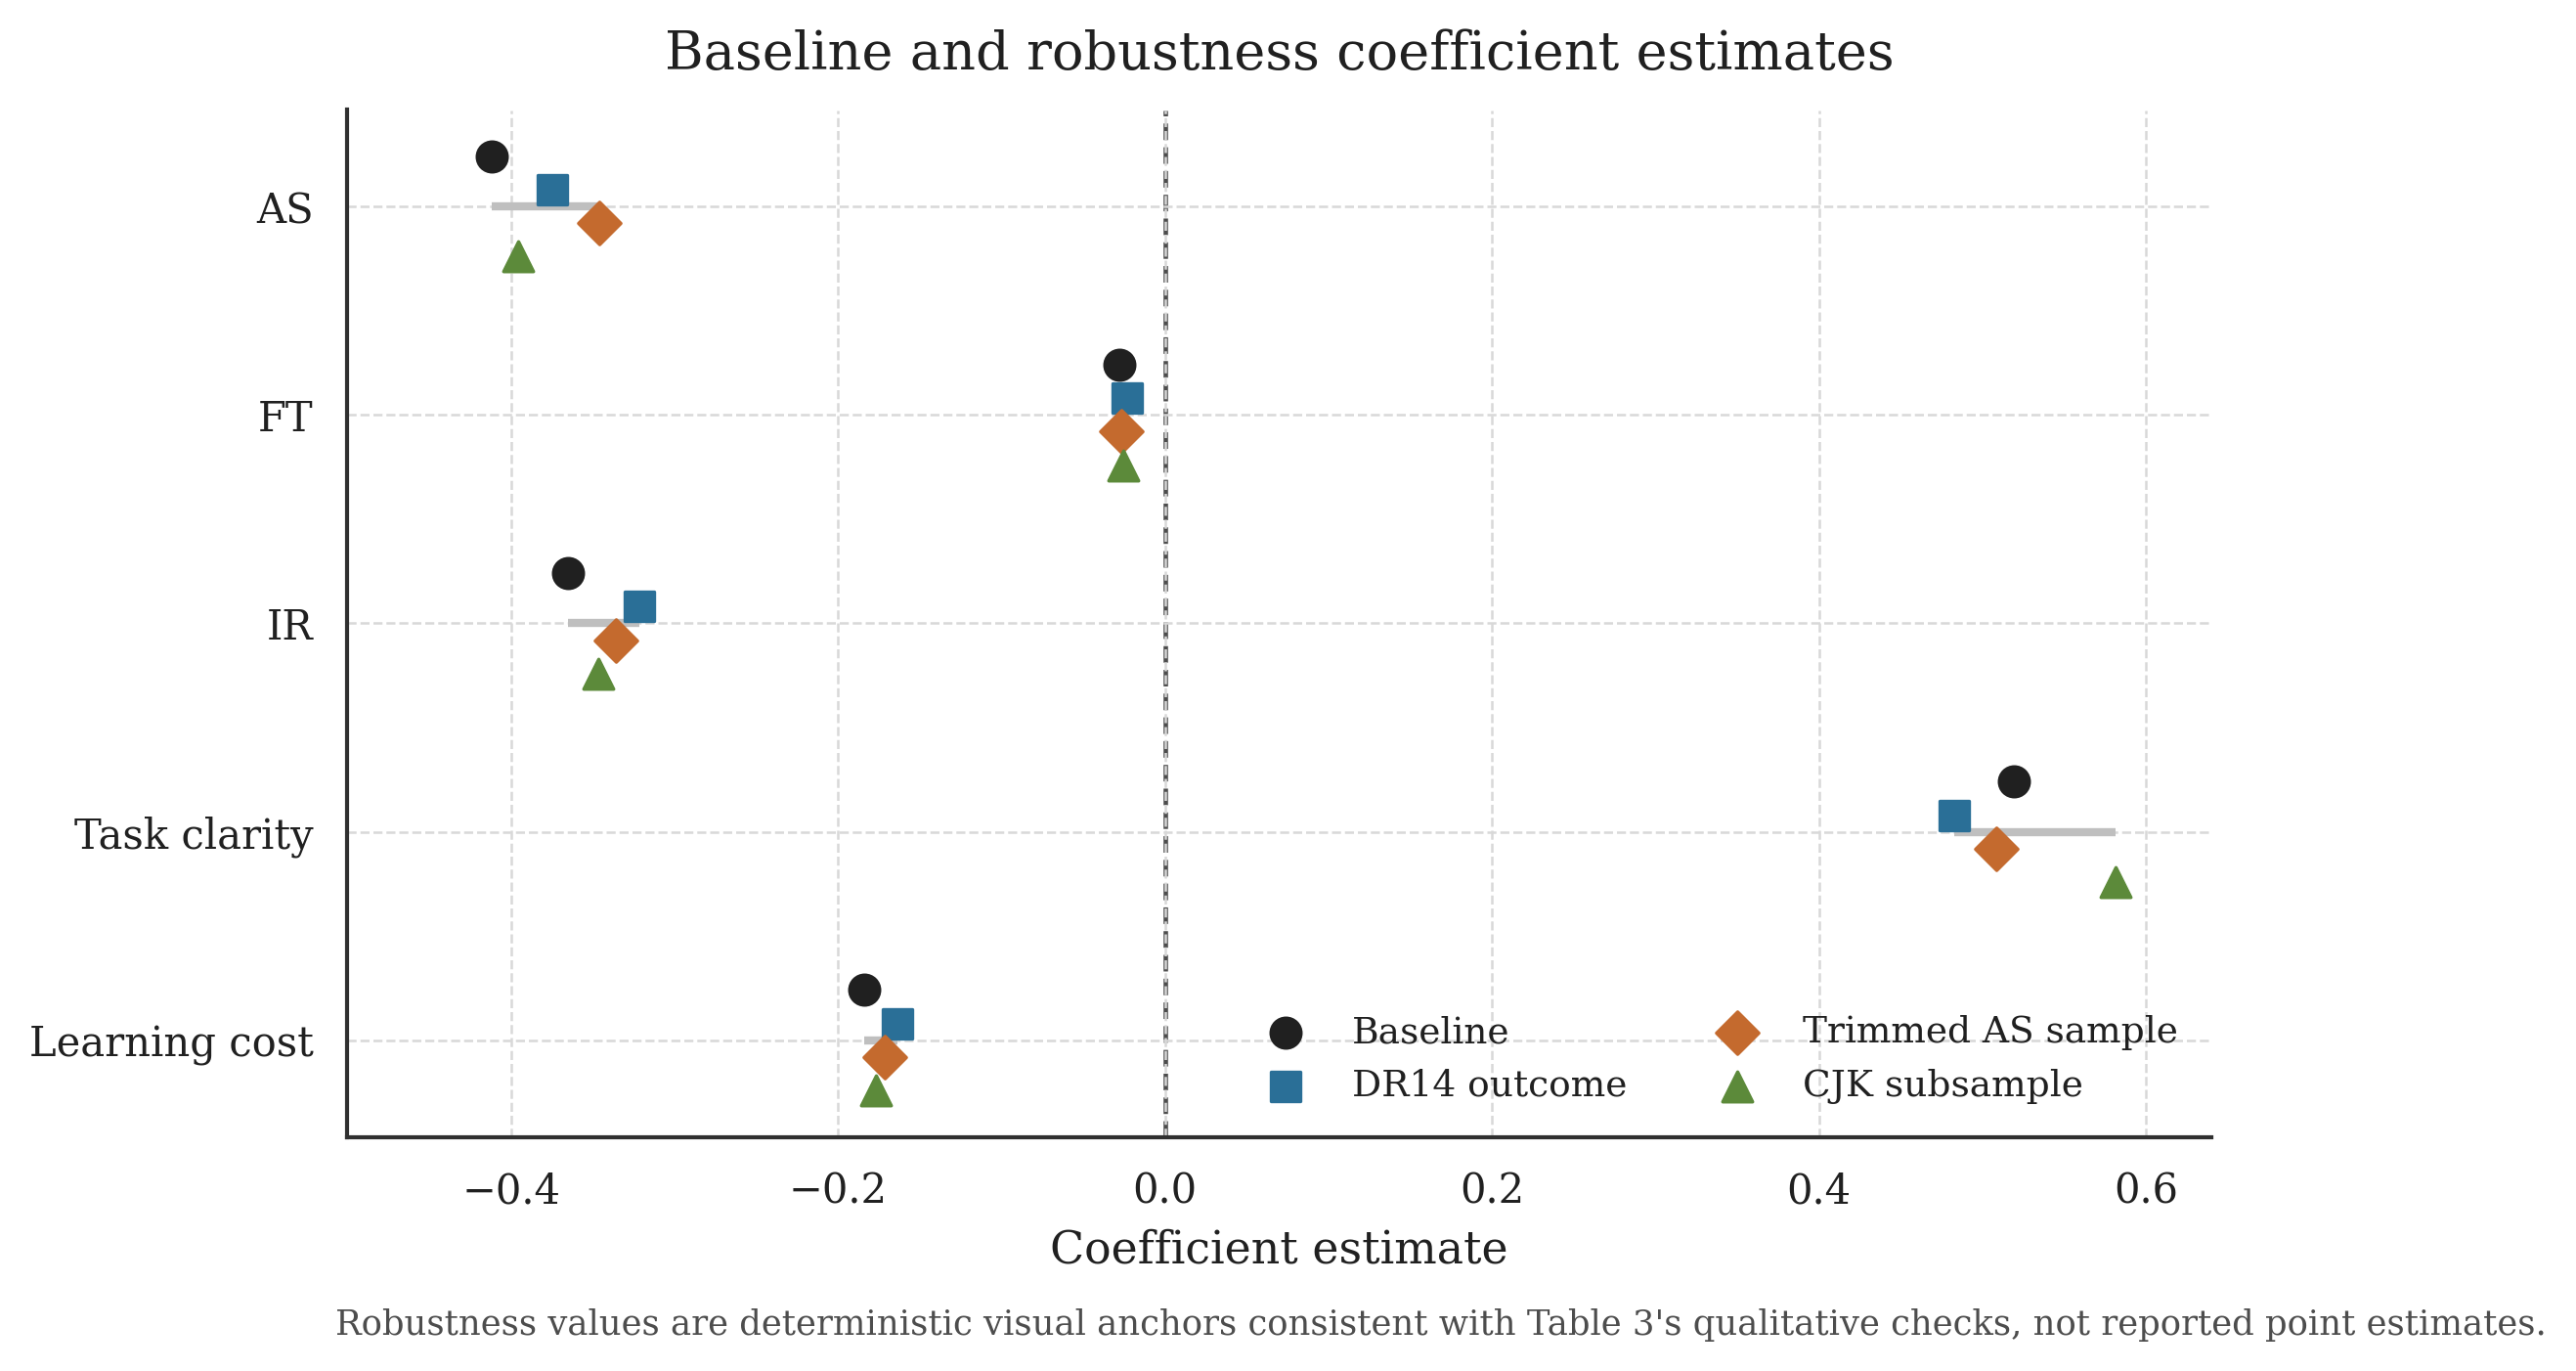
\includegraphics[width=0.95\columnwidth]{figures/fig4_robustness_coefficients.png}
\caption{稳健性系数对比}
\end{figure}

\section{CRITICAL DISCUSSION / 批判性讨论}
首先，AI 跟风热潮并不完全是“用户不理性”。它是平台机制、组织 KPI 与身份焦虑共同制造的结果。平台奖励可见性，组织奖励“已部署”叙事，个体自然会把精力投向更容易被看见的行为。

其次，“全民 all-in”常常掩盖劳动分工的现实。并不是每个人都需要成为 prompt engineer。有人需要稳定执行，有人需要复杂判断，有人需要深度协作。把同一套 AI 采用节奏强加给所有岗位，本身就是低效。

第三，技术狂热常把“不用 AI”污名化为落后。但在许多任务中，低技术方案更稳、更可审计、更少错误链。真正成熟的组织不是“全员同速”，而是允许多种技术路径并存。

\begin{quote}
\textit{适合自己的，才是高效的。不是你服务技术潮流，而是技术服务你的任务边界。}
\end{quote}

因此，我们建议把叙事从“你接了没有”改为“你复用了没有”；从“演示成功”改为“失败后能否修复”；从“热度”改为“交付”。这不是反技术，而是把技术还给现实。

\section{CONCLUSION / 结论}
AI 可以接触，但没必要狂信。工具应当进入你的工作，不必接管你的价值判断。真正的分化，不在于谁先晒截图，而在于谁能把一次成功变成可重复流程。

如果你能清楚回答这三个问题——“我在解决什么任务？”“我愿意承担什么学习成本？”“我是否得到了稳定收益？”——你就已经比热潮更清醒。

\vspace{1em}
\begin{center}
\colorbox{red!70}{\parbox{0.95\linewidth}{\centering\color{white}\bfseries 本内容纯属整活，不代表任何学术观点或现实指导建议。请保持理智，切勿模仿。}}
\end{center}

\end{document}
